\documentclass[twoside]{book}

% Packages required by doxygen
\usepackage{fixltx2e}
\usepackage{calc}
\usepackage{doxygen}
\usepackage[export]{adjustbox} % also loads graphicx
\usepackage{graphicx}
\usepackage[utf8]{inputenc}
\usepackage{makeidx}
\usepackage{multicol}
\usepackage{multirow}
\PassOptionsToPackage{warn}{textcomp}
\usepackage{textcomp}
\usepackage[nointegrals]{wasysym}
\usepackage[table]{xcolor}

% Font selection
\usepackage[T1]{fontenc}
\usepackage[scaled=.90]{helvet}
\usepackage{courier}
\usepackage{amssymb}
\usepackage{sectsty}
\renewcommand{\familydefault}{\sfdefault}
\allsectionsfont{%
  \fontseries{bc}\selectfont%
  \color{darkgray}%
}
\renewcommand{\DoxyLabelFont}{%
  \fontseries{bc}\selectfont%
  \color{darkgray}%
}
\newcommand{\+}{\discretionary{\mbox{\scriptsize$\hookleftarrow$}}{}{}}

% Page & text layout
\usepackage{geometry}
\geometry{%
  a4paper,%
  top=2.5cm,%
  bottom=2.5cm,%
  left=2.5cm,%
  right=2.5cm%
}
\tolerance=750
\hfuzz=15pt
\hbadness=750
\setlength{\emergencystretch}{15pt}
\setlength{\parindent}{0cm}
\setlength{\parskip}{3ex plus 2ex minus 2ex}
\makeatletter
\renewcommand{\paragraph}{%
  \@startsection{paragraph}{4}{0ex}{-1.0ex}{1.0ex}{%
    \normalfont\normalsize\bfseries\SS@parafont%
  }%
}
\renewcommand{\subparagraph}{%
  \@startsection{subparagraph}{5}{0ex}{-1.0ex}{1.0ex}{%
    \normalfont\normalsize\bfseries\SS@subparafont%
  }%
}
\makeatother

% Headers & footers
\usepackage{fancyhdr}
\pagestyle{fancyplain}
\fancyhead[LE]{\fancyplain{}{\bfseries\thepage}}
\fancyhead[CE]{\fancyplain{}{}}
\fancyhead[RE]{\fancyplain{}{\bfseries\leftmark}}
\fancyhead[LO]{\fancyplain{}{\bfseries\rightmark}}
\fancyhead[CO]{\fancyplain{}{}}
\fancyhead[RO]{\fancyplain{}{\bfseries\thepage}}
\fancyfoot[LE]{\fancyplain{}{}}
\fancyfoot[CE]{\fancyplain{}{}}
\fancyfoot[RE]{\fancyplain{}{\bfseries\scriptsize Generated by Doxygen }}
\fancyfoot[LO]{\fancyplain{}{\bfseries\scriptsize Generated by Doxygen }}
\fancyfoot[CO]{\fancyplain{}{}}
\fancyfoot[RO]{\fancyplain{}{}}
\renewcommand{\footrulewidth}{0.4pt}
\renewcommand{\chaptermark}[1]{%
  \markboth{#1}{}%
}
\renewcommand{\sectionmark}[1]{%
  \markright{\thesection\ #1}%
}

% Indices & bibliography
\usepackage{natbib}
\usepackage[titles]{tocloft}
\setcounter{tocdepth}{3}
\setcounter{secnumdepth}{5}
\makeindex

% Hyperlinks (required, but should be loaded last)
\usepackage{ifpdf}
\ifpdf
  \usepackage[pdftex,pagebackref=true]{hyperref}
\else
  \usepackage[ps2pdf,pagebackref=true]{hyperref}
\fi
\hypersetup{%
  colorlinks=true,%
  linkcolor=blue,%
  citecolor=blue,%
  unicode%
}

% Custom commands
\newcommand{\clearemptydoublepage}{%
  \newpage{\pagestyle{empty}\cleardoublepage}%
}

\usepackage{caption}
\captionsetup{labelsep=space,justification=centering,font={bf},singlelinecheck=off,skip=4pt,position=top}

%===== C O N T E N T S =====

\begin{document}

% Titlepage & ToC
\hypersetup{pageanchor=false,
             bookmarksnumbered=true,
             pdfencoding=unicode
            }
\pagenumbering{alph}
\begin{titlepage}
\vspace*{7cm}
\begin{center}%
{\Large unity-\/keymodule-\/wrapper }\\
\vspace*{1cm}
{\large Generated by Doxygen 1.8.14}\\
\end{center}
\end{titlepage}
\clearemptydoublepage
\pagenumbering{roman}
\tableofcontents
\clearemptydoublepage
\pagenumbering{arabic}
\hypersetup{pageanchor=true}

%--- Begin generated contents ---
\chapter{Namespace Index}
\section{Packages}
Here are the packages with brief descriptions (if available)\+:\begin{DoxyCompactList}
\item\contentsline{section}{\mbox{\hyperlink{namespace_siege_module}{Siege\+Module}} }{\pageref{namespace_siege_module}}{}
\end{DoxyCompactList}

\chapter{Hierarchical Index}
\section{Class Hierarchy}
This inheritance list is sorted roughly, but not completely, alphabetically\+:\begin{DoxyCompactList}
\item Exception\begin{DoxyCompactList}
\item \contentsline{section}{Siege\+Module.\+Uni\+Key\+Module\+Exception}{\pageref{class_siege_module_1_1_uni_key_module_exception}}{}
\end{DoxyCompactList}
\item I\+Postprocess\+Build\begin{DoxyCompactList}
\item \contentsline{section}{Siege\+Module.\+Uni\+Key\+Module\+Build\+Processor}{\pageref{class_siege_module_1_1_uni_key_module_build_processor}}{}
\end{DoxyCompactList}
\item \contentsline{section}{Siege\+Module.\+Uni\+Key\+Module\+Other.\+KV}{\pageref{struct_siege_module_1_1_uni_key_module_other_1_1_k_v}}{}
\item \contentsline{section}{L\+U\+Keychain\+Access()}{\pageref{category_l_u_keychain_access_07_08}}{}
\item N\+S\+Object\begin{DoxyCompactList}
\item \contentsline{section}{L\+U\+Keychain\+Access}{\pageref{interface_l_u_keychain_access}}{}
\item \contentsline{section}{L\+U\+Keychain\+Services}{\pageref{interface_l_u_keychain_services}}{}
\item \contentsline{section}{Uni\+Key\+Module}{\pageref{interface_uni_key_module}}{}
\end{DoxyCompactList}
\item $<$N\+S\+Object$>$\begin{DoxyCompactList}
\item \contentsline{section}{$<$L\+U\+Keychain\+Error\+Handler $>$}{\pageref{protocol_l_u_keychain_error_handler_01-p}}{}
\end{DoxyCompactList}
\item $<$N\+S\+Object\+L\+U\+Keychain\+Error\+Handler$>$\begin{DoxyCompactList}
\item \contentsline{section}{Uni\+Key\+Module()}{\pageref{category_uni_key_module_07_08}}{}
\end{DoxyCompactList}
\item \contentsline{section}{Siege\+Module.\+Uni\+Key\+Module}{\pageref{class_siege_module_1_1_uni_key_module}}{}
\item \contentsline{section}{Uni\+Key\+Module\+Boolean}{\pageref{struct_uni_key_module_boolean}}{}
\item \contentsline{section}{Siege\+Module.\+Uni\+Key\+Module\+Boolean}{\pageref{struct_siege_module_1_1_uni_key_module_boolean}}{}
\item \contentsline{section}{Siege\+Module.\+Uni\+Key\+Module\+Other}{\pageref{class_siege_module_1_1_uni_key_module_other}}{}
\item \contentsline{section}{Siege\+Module.\+Uni\+Key\+Module\+String}{\pageref{struct_siege_module_1_1_uni_key_module_string}}{}
\item \contentsline{section}{Uni\+Key\+Module\+String}{\pageref{struct_uni_key_module_string}}{}
\end{DoxyCompactList}

\chapter{Class Index}
\section{Class List}
Here are the classes, structs, unions and interfaces with brief descriptions\+:\begin{DoxyCompactList}
\item\contentsline{section}{\mbox{\hyperlink{struct_siege_module_1_1_uni_key_module_other_1_1_k_v}{Siege\+Module.\+Uni\+Key\+Module\+Other.\+KV}} \\*key-\/value data structure. }{\pageref{struct_siege_module_1_1_uni_key_module_other_1_1_k_v}}{}
\item\contentsline{section}{\mbox{\hyperlink{interface_l_u_keychain_access}{L\+U\+Keychain\+Access}} }{\pageref{interface_l_u_keychain_access}}{}
\item\contentsline{section}{\mbox{\hyperlink{category_l_u_keychain_access_07_08}{L\+U\+Keychain\+Access()}} }{\pageref{category_l_u_keychain_access_07_08}}{}
\item\contentsline{section}{\mbox{\hyperlink{protocol_l_u_keychain_error_handler_01-p}{$<$\+L\+U\+Keychain\+Error\+Handler $>$}} }{\pageref{protocol_l_u_keychain_error_handler_01-p}}{}
\item\contentsline{section}{\mbox{\hyperlink{interface_l_u_keychain_services}{L\+U\+Keychain\+Services}} }{\pageref{interface_l_u_keychain_services}}{}
\item\contentsline{section}{\mbox{\hyperlink{interface_uni_key_module}{Uni\+Key\+Module}} }{\pageref{interface_uni_key_module}}{}
\item\contentsline{section}{\mbox{\hyperlink{class_siege_module_1_1_uni_key_module}{Siege\+Module.\+Uni\+Key\+Module}} }{\pageref{class_siege_module_1_1_uni_key_module}}{}
\item\contentsline{section}{\mbox{\hyperlink{category_uni_key_module_07_08}{Uni\+Key\+Module()}} }{\pageref{category_uni_key_module_07_08}}{}
\item\contentsline{section}{\mbox{\hyperlink{struct_uni_key_module_boolean}{Uni\+Key\+Module\+Boolean}} }{\pageref{struct_uni_key_module_boolean}}{}
\item\contentsline{section}{\mbox{\hyperlink{struct_siege_module_1_1_uni_key_module_boolean}{Siege\+Module.\+Uni\+Key\+Module\+Boolean}} }{\pageref{struct_siege_module_1_1_uni_key_module_boolean}}{}
\item\contentsline{section}{\mbox{\hyperlink{class_siege_module_1_1_uni_key_module_build_processor}{Siege\+Module.\+Uni\+Key\+Module\+Build\+Processor}} }{\pageref{class_siege_module_1_1_uni_key_module_build_processor}}{}
\item\contentsline{section}{\mbox{\hyperlink{class_siege_module_1_1_uni_key_module_exception}{Siege\+Module.\+Uni\+Key\+Module\+Exception}} \\*\mbox{\hyperlink{class_siege_module_1_1_uni_key_module}{Uni\+Key\+Module}} Original Exception }{\pageref{class_siege_module_1_1_uni_key_module_exception}}{}
\item\contentsline{section}{\mbox{\hyperlink{class_siege_module_1_1_uni_key_module_other}{Siege\+Module.\+Uni\+Key\+Module\+Other}} }{\pageref{class_siege_module_1_1_uni_key_module_other}}{}
\item\contentsline{section}{\mbox{\hyperlink{struct_siege_module_1_1_uni_key_module_string}{Siege\+Module.\+Uni\+Key\+Module\+String}} }{\pageref{struct_siege_module_1_1_uni_key_module_string}}{}
\item\contentsline{section}{\mbox{\hyperlink{struct_uni_key_module_string}{Uni\+Key\+Module\+String}} }{\pageref{struct_uni_key_module_string}}{}
\end{DoxyCompactList}

\chapter{Namespace Documentation}
\hypertarget{namespace_siege_module}{}\section{Siege\+Module Namespace Reference}
\label{namespace_siege_module}\index{Siege\+Module@{Siege\+Module}}
\subsection*{Classes}
\begin{DoxyCompactItemize}
\item 
class \mbox{\hyperlink{class_siege_module_1_1_uni_key_module}{Uni\+Key\+Module}}
\item 
struct \mbox{\hyperlink{struct_siege_module_1_1_uni_key_module_boolean}{Uni\+Key\+Module\+Boolean}}
\item 
class \mbox{\hyperlink{class_siege_module_1_1_uni_key_module_build_processor}{Uni\+Key\+Module\+Build\+Processor}}
\item 
class \mbox{\hyperlink{class_siege_module_1_1_uni_key_module_exception}{Uni\+Key\+Module\+Exception}}
\begin{DoxyCompactList}\small\item\em \mbox{\hyperlink{class_siege_module_1_1_uni_key_module}{Uni\+Key\+Module}} Original Exception \end{DoxyCompactList}\item 
class \mbox{\hyperlink{class_siege_module_1_1_uni_key_module_other}{Uni\+Key\+Module\+Other}}
\item 
struct \mbox{\hyperlink{struct_siege_module_1_1_uni_key_module_string}{Uni\+Key\+Module\+String}}
\end{DoxyCompactItemize}
\subsection*{Enumerations}
\begin{DoxyCompactItemize}
\item 
\mbox{\Hypertarget{namespace_siege_module_a9dfa994d8f593ddbe2dbfec0b829d3da}\label{namespace_siege_module_a9dfa994d8f593ddbe2dbfec0b829d3da}} 
enum {\bfseries Error\+Code} \{ {\bfseries None} = 0, 
{\bfseries Unknown} = -\/1, 
{\bfseries Item\+Not\+Found} = 1
 \}
\end{DoxyCompactItemize}

\chapter{Class Documentation}
\hypertarget{struct_siege_module_1_1_uni_key_module_other_1_1_k_v}{}\section{Siege\+Module.\+Uni\+Key\+Module\+Other.\+KV Struct Reference}
\label{struct_siege_module_1_1_uni_key_module_other_1_1_k_v}\index{Siege\+Module.\+Uni\+Key\+Module\+Other.\+KV@{Siege\+Module.\+Uni\+Key\+Module\+Other.\+KV}}


key-\/value data structure.  


\subsection*{Public Member Functions}
\begin{DoxyCompactItemize}
\item 
\mbox{\hyperlink{struct_siege_module_1_1_uni_key_module_other_1_1_k_v_a70834c2e95d2cf14082fdcbef87c497b}{KV}} (string \mbox{\hyperlink{struct_siege_module_1_1_uni_key_module_other_1_1_k_v_ab66e165182f676a415d7800fa951e863}{key}}, string \mbox{\hyperlink{struct_siege_module_1_1_uni_key_module_other_1_1_k_v_a9c5e6ad07d2f59f4e7258904bc56d96d}{value}})
\begin{DoxyCompactList}\small\item\em constructor \end{DoxyCompactList}\end{DoxyCompactItemize}
\subsection*{Public Attributes}
\begin{DoxyCompactItemize}
\item 
string \mbox{\hyperlink{struct_siege_module_1_1_uni_key_module_other_1_1_k_v_ab66e165182f676a415d7800fa951e863}{key}}
\begin{DoxyCompactList}\small\item\em key \end{DoxyCompactList}\item 
string \mbox{\hyperlink{struct_siege_module_1_1_uni_key_module_other_1_1_k_v_a9c5e6ad07d2f59f4e7258904bc56d96d}{value}}
\begin{DoxyCompactList}\small\item\em value \end{DoxyCompactList}\end{DoxyCompactItemize}


\subsection{Detailed Description}
key-\/value data structure. 



\subsection{Constructor \& Destructor Documentation}
\mbox{\Hypertarget{struct_siege_module_1_1_uni_key_module_other_1_1_k_v_a70834c2e95d2cf14082fdcbef87c497b}\label{struct_siege_module_1_1_uni_key_module_other_1_1_k_v_a70834c2e95d2cf14082fdcbef87c497b}} 
\index{Siege\+Module\+::\+Uni\+Key\+Module\+Other\+::\+KV@{Siege\+Module\+::\+Uni\+Key\+Module\+Other\+::\+KV}!KV@{KV}}
\index{KV@{KV}!Siege\+Module\+::\+Uni\+Key\+Module\+Other\+::\+KV@{Siege\+Module\+::\+Uni\+Key\+Module\+Other\+::\+KV}}
\subsubsection{\texorpdfstring{K\+V()}{KV()}}
{\footnotesize\ttfamily Siege\+Module.\+Uni\+Key\+Module\+Other.\+K\+V.\+KV (\begin{DoxyParamCaption}\item[{string}]{key,  }\item[{string}]{value }\end{DoxyParamCaption})}



constructor 



\subsection{Member Data Documentation}
\mbox{\Hypertarget{struct_siege_module_1_1_uni_key_module_other_1_1_k_v_ab66e165182f676a415d7800fa951e863}\label{struct_siege_module_1_1_uni_key_module_other_1_1_k_v_ab66e165182f676a415d7800fa951e863}} 
\index{Siege\+Module\+::\+Uni\+Key\+Module\+Other\+::\+KV@{Siege\+Module\+::\+Uni\+Key\+Module\+Other\+::\+KV}!key@{key}}
\index{key@{key}!Siege\+Module\+::\+Uni\+Key\+Module\+Other\+::\+KV@{Siege\+Module\+::\+Uni\+Key\+Module\+Other\+::\+KV}}
\subsubsection{\texorpdfstring{key}{key}}
{\footnotesize\ttfamily string Siege\+Module.\+Uni\+Key\+Module\+Other.\+K\+V.\+key}



key 

\mbox{\Hypertarget{struct_siege_module_1_1_uni_key_module_other_1_1_k_v_a9c5e6ad07d2f59f4e7258904bc56d96d}\label{struct_siege_module_1_1_uni_key_module_other_1_1_k_v_a9c5e6ad07d2f59f4e7258904bc56d96d}} 
\index{Siege\+Module\+::\+Uni\+Key\+Module\+Other\+::\+KV@{Siege\+Module\+::\+Uni\+Key\+Module\+Other\+::\+KV}!value@{value}}
\index{value@{value}!Siege\+Module\+::\+Uni\+Key\+Module\+Other\+::\+KV@{Siege\+Module\+::\+Uni\+Key\+Module\+Other\+::\+KV}}
\subsubsection{\texorpdfstring{value}{value}}
{\footnotesize\ttfamily string Siege\+Module.\+Uni\+Key\+Module\+Other.\+K\+V.\+value}



value 



The documentation for this struct was generated from the following file\+:\begin{DoxyCompactItemize}
\item 
Assets/\+Plugins/unikeymodule/\+Other/Uni\+Key\+Module\+Other.\+cs\end{DoxyCompactItemize}

\hypertarget{interface_l_u_keychain_access}{}\section{L\+U\+Keychain\+Access Class Reference}
\label{interface_l_u_keychain_access}\index{L\+U\+Keychain\+Access@{L\+U\+Keychain\+Access}}
Inheritance diagram for L\+U\+Keychain\+Access\+:\begin{figure}[H]
\begin{center}
\leavevmode
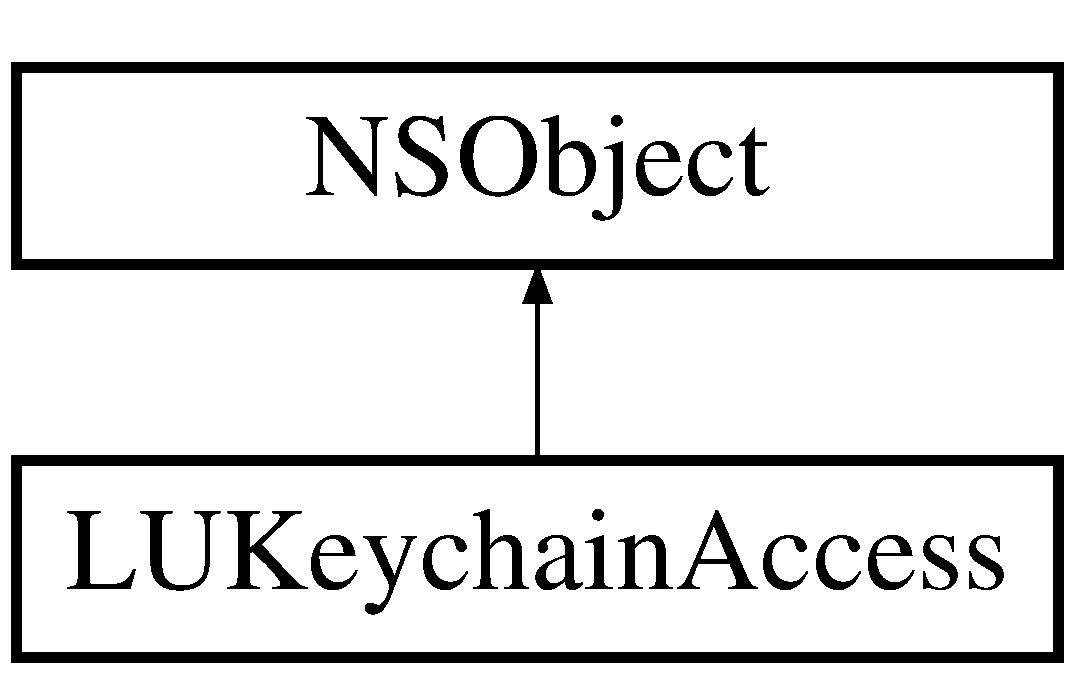
\includegraphics[height=2.000000cm]{interface_l_u_keychain_access}
\end{center}
\end{figure}
\subsection*{Instance Methods}
\begin{DoxyCompactItemize}
\item 
\mbox{\Hypertarget{interface_l_u_keychain_access_aac0c41c0a0bc247698439c0d3507989a}\label{interface_l_u_keychain_access_aac0c41c0a0bc247698439c0d3507989a}} 
(B\+O\+OL) -\/ {\bfseries delete\+All}
\item 
\mbox{\Hypertarget{interface_l_u_keychain_access_a314f2e35b0b3fa6731a0b54b71c054e2}\label{interface_l_u_keychain_access_a314f2e35b0b3fa6731a0b54b71c054e2}} 
(void) -\/ {\bfseries delete\+Object\+For\+Key\+:}
\item 
\mbox{\Hypertarget{interface_l_u_keychain_access_abce18a99a89dd5962cc5dacce5feb3ac}\label{interface_l_u_keychain_access_abce18a99a89dd5962cc5dacce5feb3ac}} 
(B\+O\+OL) -\/ {\bfseries bool\+For\+Key\+:}
\item 
\mbox{\Hypertarget{interface_l_u_keychain_access_ab73f8f3bc71d093632c5165f3372a8dd}\label{interface_l_u_keychain_access_ab73f8f3bc71d093632c5165f3372a8dd}} 
(nullable N\+S\+Data $\ast$) -\/ {\bfseries data\+For\+Key\+:}
\item 
\mbox{\Hypertarget{interface_l_u_keychain_access_acb107263130a9a418e89be6d2b8df375}\label{interface_l_u_keychain_access_acb107263130a9a418e89be6d2b8df375}} 
(double) -\/ {\bfseries double\+For\+Key\+:}
\item 
\mbox{\Hypertarget{interface_l_u_keychain_access_acc5f251af8cd676a315b9031b048631f}\label{interface_l_u_keychain_access_acc5f251af8cd676a315b9031b048631f}} 
(float) -\/ {\bfseries float\+For\+Key\+:}
\item 
\mbox{\Hypertarget{interface_l_u_keychain_access_a81791dacaa240e789d57814d0123b2da}\label{interface_l_u_keychain_access_a81791dacaa240e789d57814d0123b2da}} 
(N\+S\+Integer) -\/ {\bfseries integer\+For\+Key\+:}
\item 
\mbox{\Hypertarget{interface_l_u_keychain_access_a33501dd8e3a7fbe1427b4e4f8caceaea}\label{interface_l_u_keychain_access_a33501dd8e3a7fbe1427b4e4f8caceaea}} 
(nullable id) -\/ {\bfseries object\+For\+Key\+:}
\item 
\mbox{\Hypertarget{interface_l_u_keychain_access_a26cc0ff686e8f29d5f5934b0318a2205}\label{interface_l_u_keychain_access_a26cc0ff686e8f29d5f5934b0318a2205}} 
(nullable N\+S\+String $\ast$) -\/ {\bfseries string\+For\+Key\+:}
\item 
\mbox{\Hypertarget{interface_l_u_keychain_access_a850de511433de921e83f52f206c374b3}\label{interface_l_u_keychain_access_a850de511433de921e83f52f206c374b3}} 
(void) -\/ {\bfseries register\+Defaults\+:}
\item 
\mbox{\Hypertarget{interface_l_u_keychain_access_a4c1ba958e1dd4a1559d845b31ed36df4}\label{interface_l_u_keychain_access_a4c1ba958e1dd4a1559d845b31ed36df4}} 
(void) -\/ {\bfseries set\+Bool\+:for\+Key\+:}
\item 
\mbox{\Hypertarget{interface_l_u_keychain_access_ae32caf83e921c65b3567b533bdf5d0a4}\label{interface_l_u_keychain_access_ae32caf83e921c65b3567b533bdf5d0a4}} 
(void) -\/ {\bfseries set\+Data\+:for\+Key\+:}
\item 
\mbox{\Hypertarget{interface_l_u_keychain_access_afcce38895ac6bb83376d8593c43be091}\label{interface_l_u_keychain_access_afcce38895ac6bb83376d8593c43be091}} 
(void) -\/ {\bfseries set\+Double\+:for\+Key\+:}
\item 
\mbox{\Hypertarget{interface_l_u_keychain_access_a322aaed1cda576f5bcf1b843a1235832}\label{interface_l_u_keychain_access_a322aaed1cda576f5bcf1b843a1235832}} 
(void) -\/ {\bfseries set\+Float\+:for\+Key\+:}
\item 
\mbox{\Hypertarget{interface_l_u_keychain_access_a5520fe6ace25f9837d36ae35e62371c5}\label{interface_l_u_keychain_access_a5520fe6ace25f9837d36ae35e62371c5}} 
(void) -\/ {\bfseries set\+Integer\+:for\+Key\+:}
\item 
\mbox{\Hypertarget{interface_l_u_keychain_access_ab49b6ef651d8b56dc619a6afed4e690a}\label{interface_l_u_keychain_access_ab49b6ef651d8b56dc619a6afed4e690a}} 
(void) -\/ {\bfseries set\+Object\+:for\+Key\+:}
\item 
\mbox{\Hypertarget{interface_l_u_keychain_access_a006449f86f8aa4de492d7c61ac027a54}\label{interface_l_u_keychain_access_a006449f86f8aa4de492d7c61ac027a54}} 
(void) -\/ {\bfseries set\+String\+:for\+Key\+:}
\end{DoxyCompactItemize}
\subsection*{Class Methods}
\begin{DoxyCompactItemize}
\item 
\mbox{\Hypertarget{interface_l_u_keychain_access_a31f4824d67c9f76192008a8fc7ae7b73}\label{interface_l_u_keychain_access_a31f4824d67c9f76192008a8fc7ae7b73}} 
(\mbox{\hyperlink{interface_l_u_keychain_access}{L\+U\+Keychain\+Access}} $\ast$) + {\bfseries standard\+Keychain\+Access}
\end{DoxyCompactItemize}
\subsection*{Properties}
\begin{DoxyCompactItemize}
\item 
\mbox{\Hypertarget{interface_l_u_keychain_access_adc9ae3c1ac74d700df0ca3ccae4a5a34}\label{interface_l_u_keychain_access_adc9ae3c1ac74d700df0ca3ccae4a5a34}} 
N\+S\+String $\ast$ {\bfseries access\+Group}
\item 
\mbox{\Hypertarget{interface_l_u_keychain_access_a8b0f24a0ed9b9138dcfcace353d99e00}\label{interface_l_u_keychain_access_a8b0f24a0ed9b9138dcfcace353d99e00}} 
L\+U\+Keychain\+Access\+Accessibility {\bfseries accessibility\+State}
\item 
\mbox{\Hypertarget{interface_l_u_keychain_access_acc5b5f576850765ec8964fc955005a08}\label{interface_l_u_keychain_access_acc5b5f576850765ec8964fc955005a08}} 
id$<$ L\+U\+Keychain\+Error\+Handler $>$ {\bfseries error\+Handler}
\item 
\mbox{\Hypertarget{interface_l_u_keychain_access_a09dff710bf73e789518b04c664469624}\label{interface_l_u_keychain_access_a09dff710bf73e789518b04c664469624}} 
N\+S\+String $\ast$ {\bfseries service}
\end{DoxyCompactItemize}


The documentation for this class was generated from the following files\+:\begin{DoxyCompactItemize}
\item 
Assets/\+Plugins/unikeymodule/i\+O\+S/\+L\+U\+Keychain\+Access/L\+U\+Keychain\+Access.\+h\item 
Assets/\+Plugins/unikeymodule/i\+O\+S/\+L\+U\+Keychain\+Access/L\+U\+Keychain\+Access.\+m\end{DoxyCompactItemize}

\hypertarget{category_l_u_keychain_access_07_08}{}\section{L\+U\+Keychain\+Access() Category Reference}
\label{category_l_u_keychain_access_07_08}\index{L\+U\+Keychain\+Access()@{L\+U\+Keychain\+Access()}}
\subsection*{Properties}
\begin{DoxyCompactItemize}
\item 
\mbox{\Hypertarget{category_l_u_keychain_access_07_08_abacce8eac8ea9d7ae7e85cf0a1ba15e7}\label{category_l_u_keychain_access_07_08_abacce8eac8ea9d7ae7e85cf0a1ba15e7}} 
\mbox{\hyperlink{interface_l_u_keychain_services}{L\+U\+Keychain\+Services}} $\ast$ {\bfseries keychain\+Services}
\end{DoxyCompactItemize}


The documentation for this category was generated from the following file\+:\begin{DoxyCompactItemize}
\item 
Assets/\+Plugins/unikeymodule/i\+O\+S/\+L\+U\+Keychain\+Access/L\+U\+Keychain\+Access.\+m\end{DoxyCompactItemize}

\hypertarget{protocol_l_u_keychain_error_handler_01-p}{}\section{$<$L\+U\+Keychain\+Error\+Handler $>$ Protocol Reference}
\label{protocol_l_u_keychain_error_handler_01-p}\index{$<$\+L\+U\+Keychain\+Error\+Handler $>$@{$<$\+L\+U\+Keychain\+Error\+Handler $>$}}
Inheritance diagram for $<$L\+U\+Keychain\+Error\+Handler $>$\+:\begin{figure}[H]
\begin{center}
\leavevmode
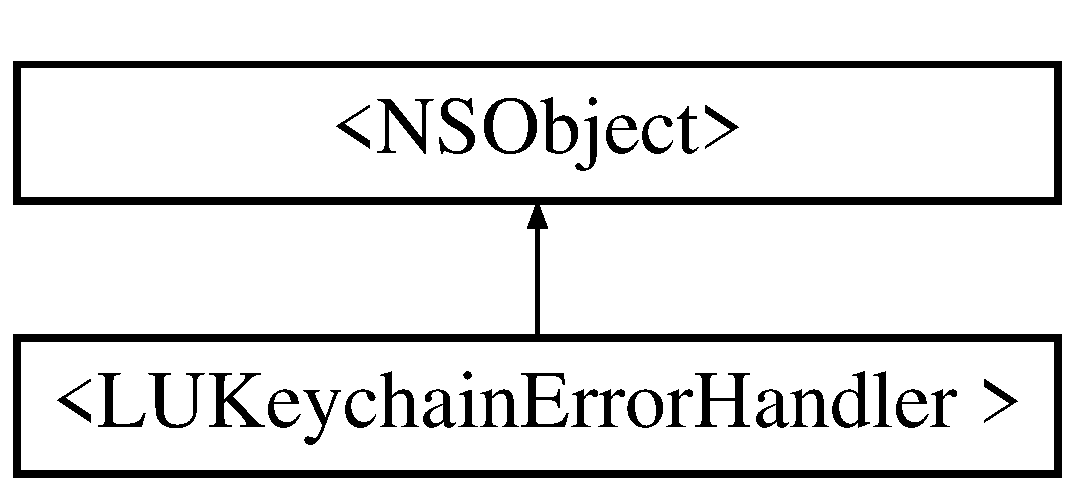
\includegraphics[height=2.000000cm]{protocol_l_u_keychain_error_handler_01-p}
\end{center}
\end{figure}
\subsection*{Instance Methods}
\begin{DoxyCompactItemize}
\item 
\mbox{\Hypertarget{protocol_l_u_keychain_error_handler_01-p_a57aba4a7e6d1f42dd729b333a308175b}\label{protocol_l_u_keychain_error_handler_01-p_a57aba4a7e6d1f42dd729b333a308175b}} 
(void) -\/ {\bfseries keychain\+Access\+:received\+Error\+:}
\end{DoxyCompactItemize}


The documentation for this protocol was generated from the following file\+:\begin{DoxyCompactItemize}
\item 
Assets/\+Plugins/unikeymodule/i\+O\+S/\+L\+U\+Keychain\+Access/L\+U\+Keychain\+Error\+Handler.\+h\end{DoxyCompactItemize}

\hypertarget{interface_l_u_keychain_services}{}\section{L\+U\+Keychain\+Services Class Reference}
\label{interface_l_u_keychain_services}\index{L\+U\+Keychain\+Services@{L\+U\+Keychain\+Services}}
Inheritance diagram for L\+U\+Keychain\+Services\+:\begin{figure}[H]
\begin{center}
\leavevmode
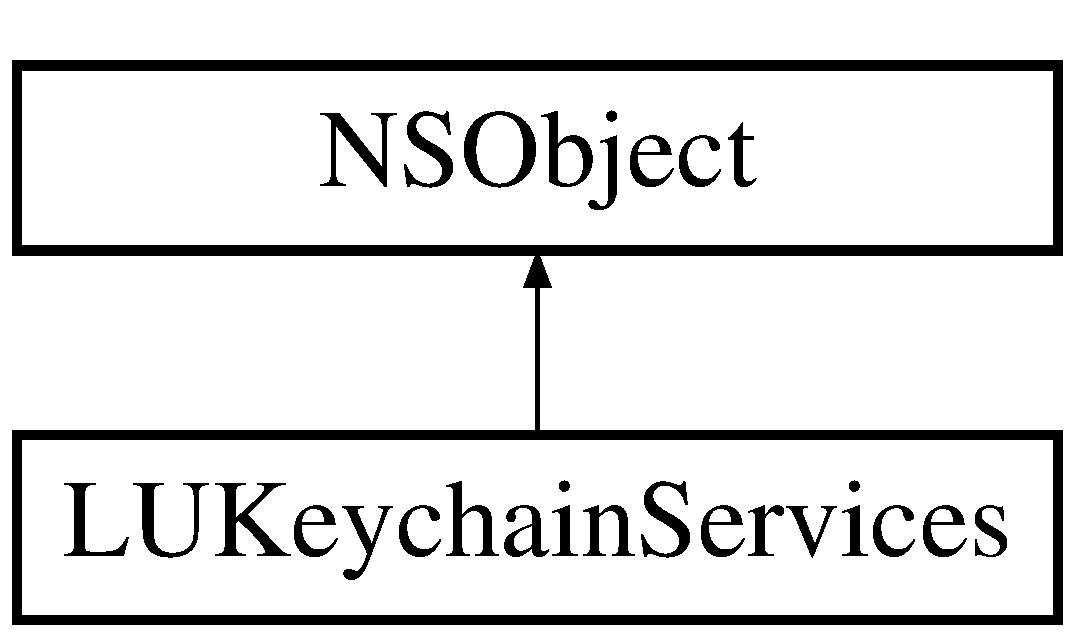
\includegraphics[height=2.000000cm]{interface_l_u_keychain_services}
\end{center}
\end{figure}
\subsection*{Instance Methods}
\begin{DoxyCompactItemize}
\item 
\mbox{\Hypertarget{interface_l_u_keychain_services_a1feccf44fa5e07b9344c41cdb9a4628f}\label{interface_l_u_keychain_services_a1feccf44fa5e07b9344c41cdb9a4628f}} 
(B\+O\+OL) -\/ {\bfseries add\+Data\+:for\+Key\+:error\+:}
\item 
\mbox{\Hypertarget{interface_l_u_keychain_services_afcc434286ce6f83cfe3d6557d7e6f588}\label{interface_l_u_keychain_services_afcc434286ce6f83cfe3d6557d7e6f588}} 
(N\+S\+Data $\ast$) -\/ {\bfseries data\+For\+Key\+:error\+:}
\item 
\mbox{\Hypertarget{interface_l_u_keychain_services_a29826893a1306714776c3abcd6348666}\label{interface_l_u_keychain_services_a29826893a1306714776c3abcd6348666}} 
(B\+O\+OL) -\/ {\bfseries delete\+All\+Items\+With\+Error\+:}
\item 
\mbox{\Hypertarget{interface_l_u_keychain_services_ac48065b3c8e6e16b66f1f429eade9c84}\label{interface_l_u_keychain_services_ac48065b3c8e6e16b66f1f429eade9c84}} 
(B\+O\+OL) -\/ {\bfseries delete\+Item\+With\+Key\+:error\+:}
\item 
\mbox{\Hypertarget{interface_l_u_keychain_services_a5cadd64c760a69004b5e7920f6c29b9e}\label{interface_l_u_keychain_services_a5cadd64c760a69004b5e7920f6c29b9e}} 
(B\+O\+OL) -\/ {\bfseries update\+Data\+:for\+Key\+:error\+:}
\end{DoxyCompactItemize}
\subsection*{Class Methods}
\begin{DoxyCompactItemize}
\item 
\mbox{\Hypertarget{interface_l_u_keychain_services_adc4ed1267d01f65481f99afbbf2a0be1}\label{interface_l_u_keychain_services_adc4ed1267d01f65481f99afbbf2a0be1}} 
(instancetype) + {\bfseries keychain\+Services}
\end{DoxyCompactItemize}
\subsection*{Properties}
\begin{DoxyCompactItemize}
\item 
\mbox{\Hypertarget{interface_l_u_keychain_services_a04052ec07298afdd22fab1827918758c}\label{interface_l_u_keychain_services_a04052ec07298afdd22fab1827918758c}} 
N\+S\+String $\ast$ {\bfseries access\+Group}
\item 
\mbox{\Hypertarget{interface_l_u_keychain_services_acd3b58dac74ff81be562b03e6cccfcf7}\label{interface_l_u_keychain_services_acd3b58dac74ff81be562b03e6cccfcf7}} 
L\+U\+Keychain\+Access\+Accessibility {\bfseries accessibility\+State}
\item 
\mbox{\Hypertarget{interface_l_u_keychain_services_afd9d562afbad040bf34f14e3bda761c0}\label{interface_l_u_keychain_services_afd9d562afbad040bf34f14e3bda761c0}} 
N\+S\+String $\ast$ {\bfseries service}
\end{DoxyCompactItemize}


The documentation for this class was generated from the following files\+:\begin{DoxyCompactItemize}
\item 
Assets/\+Plugins/unikeymodule/i\+O\+S/\+L\+U\+Keychain\+Access/L\+U\+Keychain\+Services.\+h\item 
Assets/\+Plugins/unikeymodule/i\+O\+S/\+L\+U\+Keychain\+Access/L\+U\+Keychain\+Services.\+m\end{DoxyCompactItemize}

\hypertarget{interface_uni_key_module}{}\section{Uni\+Key\+Module Class Reference}
\label{interface_uni_key_module}\index{Uni\+Key\+Module@{Uni\+Key\+Module}}
Inheritance diagram for Uni\+Key\+Module\+:\begin{figure}[H]
\begin{center}
\leavevmode
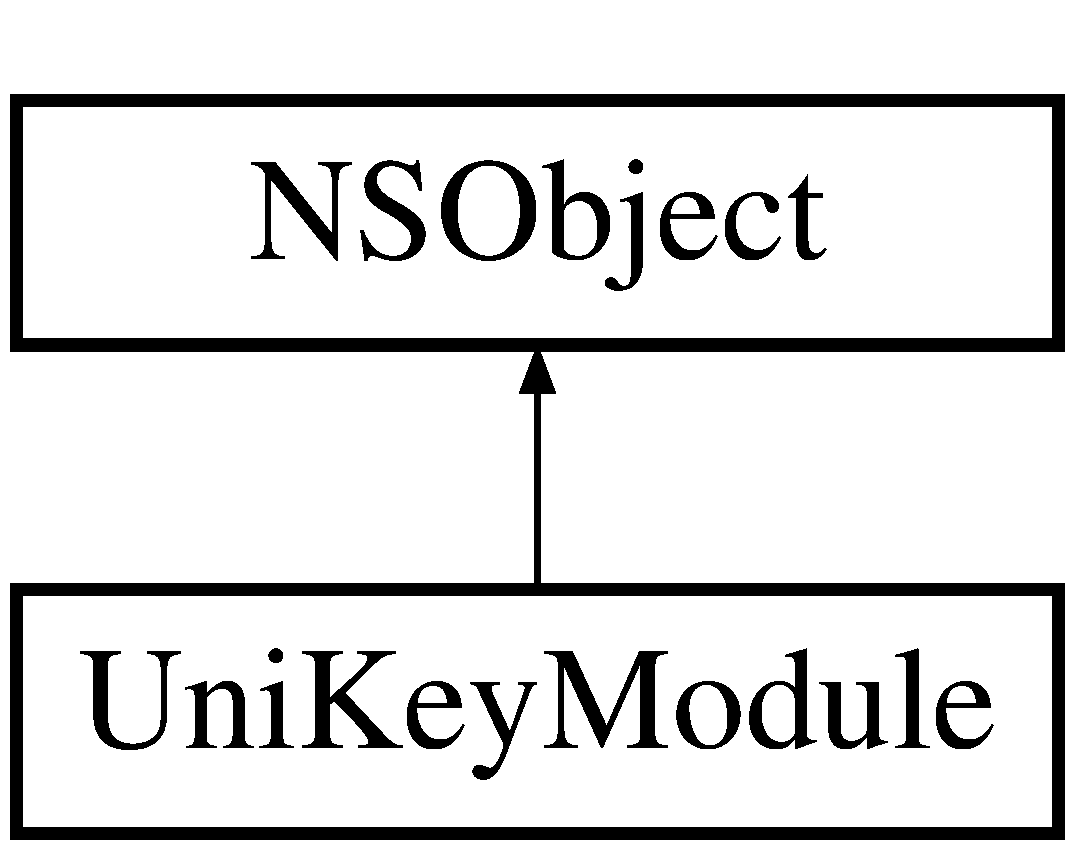
\includegraphics[height=2.000000cm]{interface_uni_key_module}
\end{center}
\end{figure}
\subsection*{Instance Methods}
\begin{DoxyCompactItemize}
\item 
(void) -\/ \mbox{\hyperlink{interface_uni_key_module_ae37bf10e6cf96ec636dcfbf5bdd8fa21}{delete\+All}}
\item 
(void) -\/ \mbox{\hyperlink{interface_uni_key_module_aa09e63616e9bf53c82d9ab230fe111b4}{delete\+Key\+:}}
\item 
(N\+S\+String $\ast$) -\/ \mbox{\hyperlink{interface_uni_key_module_ad14f35dbf0453ec2807028edc3bc5c7f}{get\+String\+:}}
\item 
(void) -\/ \mbox{\hyperlink{interface_uni_key_module_a7240067e8b706485080753c8a8a063c1}{set\+String\+:value\+:}}
\end{DoxyCompactItemize}
\subsection*{Class Methods}
\begin{DoxyCompactItemize}
\item 
(\mbox{\hyperlink{interface_uni_key_module}{Uni\+Key\+Module}} $\ast$) + \mbox{\hyperlink{interface_uni_key_module_a32a8491c21919320c2b88f1252aad3c9}{shared\+Instance}}
\end{DoxyCompactItemize}


\subsection{Method Documentation}
\mbox{\Hypertarget{interface_uni_key_module_ae37bf10e6cf96ec636dcfbf5bdd8fa21}\label{interface_uni_key_module_ae37bf10e6cf96ec636dcfbf5bdd8fa21}} 
\index{Uni\+Key\+Module@{Uni\+Key\+Module}!delete\+All@{delete\+All}}
\index{delete\+All@{delete\+All}!Uni\+Key\+Module@{Uni\+Key\+Module}}
\subsubsection{\texorpdfstring{delete\+All()}{deleteAll()}}
{\footnotesize\ttfamily -\/ (void) delete\+All \begin{DoxyParamCaption}{ }\end{DoxyParamCaption}}

remove all data from keychain. \mbox{\Hypertarget{interface_uni_key_module_aa09e63616e9bf53c82d9ab230fe111b4}\label{interface_uni_key_module_aa09e63616e9bf53c82d9ab230fe111b4}} 
\index{Uni\+Key\+Module@{Uni\+Key\+Module}!delete\+Key\+:@{delete\+Key\+:}}
\index{delete\+Key\+:@{delete\+Key\+:}!Uni\+Key\+Module@{Uni\+Key\+Module}}
\subsubsection{\texorpdfstring{delete\+Key\+:()}{deleteKey:()}}
{\footnotesize\ttfamily -\/ (void) delete\+Key\+: \begin{DoxyParamCaption}\item[{(N\+S\+String$\ast$)}]{key }\end{DoxyParamCaption}}

remove one data from keychain \mbox{\Hypertarget{interface_uni_key_module_ad14f35dbf0453ec2807028edc3bc5c7f}\label{interface_uni_key_module_ad14f35dbf0453ec2807028edc3bc5c7f}} 
\index{Uni\+Key\+Module@{Uni\+Key\+Module}!get\+String\+:@{get\+String\+:}}
\index{get\+String\+:@{get\+String\+:}!Uni\+Key\+Module@{Uni\+Key\+Module}}
\subsubsection{\texorpdfstring{get\+String\+:()}{getString:()}}
{\footnotesize\ttfamily -\/ (N\+S\+String $\ast$) get\+String\+: \begin{DoxyParamCaption}\item[{(N\+S\+String $\ast$)}]{key }\end{DoxyParamCaption}}

get data from keychain \mbox{\Hypertarget{interface_uni_key_module_a7240067e8b706485080753c8a8a063c1}\label{interface_uni_key_module_a7240067e8b706485080753c8a8a063c1}} 
\index{Uni\+Key\+Module@{Uni\+Key\+Module}!set\+String\+:value\+:@{set\+String\+:value\+:}}
\index{set\+String\+:value\+:@{set\+String\+:value\+:}!Uni\+Key\+Module@{Uni\+Key\+Module}}
\subsubsection{\texorpdfstring{set\+String\+:value\+:()}{setString:value:()}}
{\footnotesize\ttfamily -\/ (void) set\+String\+: \begin{DoxyParamCaption}\item[{(N\+S\+String $\ast$)}]{key }\item[{value:(N\+S\+String $\ast$)}]{value }\end{DoxyParamCaption}}

register or update data to keychain. \mbox{\Hypertarget{interface_uni_key_module_a32a8491c21919320c2b88f1252aad3c9}\label{interface_uni_key_module_a32a8491c21919320c2b88f1252aad3c9}} 
\index{Uni\+Key\+Module@{Uni\+Key\+Module}!shared\+Instance@{shared\+Instance}}
\index{shared\+Instance@{shared\+Instance}!Uni\+Key\+Module@{Uni\+Key\+Module}}
\subsubsection{\texorpdfstring{shared\+Instance()}{sharedInstance()}}
{\footnotesize\ttfamily + (\mbox{\hyperlink{interface_uni_key_module}{Uni\+Key\+Module}} $\ast$) shared\+Instance \begin{DoxyParamCaption}{ }\end{DoxyParamCaption}}

generate singleton instance. 

The documentation for this class was generated from the following file\+:\begin{DoxyCompactItemize}
\item 
Assets/\+Plugins/unikeymodule/i\+O\+S/Uni\+Key\+Module.\+mm\end{DoxyCompactItemize}

\hypertarget{class_siege_module_1_1_uni_key_module}{}\section{Siege\+Module.\+Uni\+Key\+Module Class Reference}
\label{class_siege_module_1_1_uni_key_module}\index{Siege\+Module.\+Uni\+Key\+Module@{Siege\+Module.\+Uni\+Key\+Module}}
\subsection*{Static Public Member Functions}
\begin{DoxyCompactItemize}
\item 
static string \mbox{\hyperlink{class_siege_module_1_1_uni_key_module_a26c856f2a81d3c561295afb1936fed37}{Get\+String}} (string key)
\begin{DoxyCompactList}\small\item\em get string from native code. \end{DoxyCompactList}\item 
static void \mbox{\hyperlink{class_siege_module_1_1_uni_key_module_ab17cd59318975668525fcf694b5dd88d}{Set\+String}} (string key, string value)
\begin{DoxyCompactList}\small\item\em set string to native code. \end{DoxyCompactList}\item 
static bool \mbox{\hyperlink{class_siege_module_1_1_uni_key_module_a55044c9eefa50b2157b1214903616fdc}{Has\+Key}} (string key)
\begin{DoxyCompactList}\small\item\em confirm that received key exists in native code. \end{DoxyCompactList}\item 
static void \mbox{\hyperlink{class_siege_module_1_1_uni_key_module_a1a14008fba02dd38b420879a97d2ed21}{Delete\+Key}} (string key)
\begin{DoxyCompactList}\small\item\em remove data which related received key in native code. \end{DoxyCompactList}\item 
static void \mbox{\hyperlink{class_siege_module_1_1_uni_key_module_a04963e00a7581e30722e42039eadb923}{Delete\+All}} ()
\begin{DoxyCompactList}\small\item\em remove all data in data store. \end{DoxyCompactList}\end{DoxyCompactItemize}


\subsection{Member Function Documentation}
\mbox{\Hypertarget{class_siege_module_1_1_uni_key_module_a04963e00a7581e30722e42039eadb923}\label{class_siege_module_1_1_uni_key_module_a04963e00a7581e30722e42039eadb923}} 
\index{Siege\+Module\+::\+Uni\+Key\+Module@{Siege\+Module\+::\+Uni\+Key\+Module}!Delete\+All@{Delete\+All}}
\index{Delete\+All@{Delete\+All}!Siege\+Module\+::\+Uni\+Key\+Module@{Siege\+Module\+::\+Uni\+Key\+Module}}
\subsubsection{\texorpdfstring{Delete\+All()}{DeleteAll()}}
{\footnotesize\ttfamily static void Siege\+Module.\+Uni\+Key\+Module.\+Delete\+All (\begin{DoxyParamCaption}{ }\end{DoxyParamCaption})\hspace{0.3cm}{\ttfamily [static]}}



remove all data in data store. 

\mbox{\Hypertarget{class_siege_module_1_1_uni_key_module_a1a14008fba02dd38b420879a97d2ed21}\label{class_siege_module_1_1_uni_key_module_a1a14008fba02dd38b420879a97d2ed21}} 
\index{Siege\+Module\+::\+Uni\+Key\+Module@{Siege\+Module\+::\+Uni\+Key\+Module}!Delete\+Key@{Delete\+Key}}
\index{Delete\+Key@{Delete\+Key}!Siege\+Module\+::\+Uni\+Key\+Module@{Siege\+Module\+::\+Uni\+Key\+Module}}
\subsubsection{\texorpdfstring{Delete\+Key()}{DeleteKey()}}
{\footnotesize\ttfamily static void Siege\+Module.\+Uni\+Key\+Module.\+Delete\+Key (\begin{DoxyParamCaption}\item[{string}]{key }\end{DoxyParamCaption})\hspace{0.3cm}{\ttfamily [static]}}



remove data which related received key in native code. 


\begin{DoxyParams}{Parameters}
{\em key} & key\\
\hline
\end{DoxyParams}
\mbox{\Hypertarget{class_siege_module_1_1_uni_key_module_a26c856f2a81d3c561295afb1936fed37}\label{class_siege_module_1_1_uni_key_module_a26c856f2a81d3c561295afb1936fed37}} 
\index{Siege\+Module\+::\+Uni\+Key\+Module@{Siege\+Module\+::\+Uni\+Key\+Module}!Get\+String@{Get\+String}}
\index{Get\+String@{Get\+String}!Siege\+Module\+::\+Uni\+Key\+Module@{Siege\+Module\+::\+Uni\+Key\+Module}}
\subsubsection{\texorpdfstring{Get\+String()}{GetString()}}
{\footnotesize\ttfamily static string Siege\+Module.\+Uni\+Key\+Module.\+Get\+String (\begin{DoxyParamCaption}\item[{string}]{key }\end{DoxyParamCaption})\hspace{0.3cm}{\ttfamily [static]}}



get string from native code. 

\begin{DoxyReturn}{Returns}
value
\end{DoxyReturn}

\begin{DoxyParams}{Parameters}
{\em key} & key\\
\hline
\end{DoxyParams}
\mbox{\Hypertarget{class_siege_module_1_1_uni_key_module_a55044c9eefa50b2157b1214903616fdc}\label{class_siege_module_1_1_uni_key_module_a55044c9eefa50b2157b1214903616fdc}} 
\index{Siege\+Module\+::\+Uni\+Key\+Module@{Siege\+Module\+::\+Uni\+Key\+Module}!Has\+Key@{Has\+Key}}
\index{Has\+Key@{Has\+Key}!Siege\+Module\+::\+Uni\+Key\+Module@{Siege\+Module\+::\+Uni\+Key\+Module}}
\subsubsection{\texorpdfstring{Has\+Key()}{HasKey()}}
{\footnotesize\ttfamily static bool Siege\+Module.\+Uni\+Key\+Module.\+Has\+Key (\begin{DoxyParamCaption}\item[{string}]{key }\end{DoxyParamCaption})\hspace{0.3cm}{\ttfamily [static]}}



confirm that received key exists in native code. 

\begin{DoxyReturn}{Returns}
whether key contains native code, or not.
\end{DoxyReturn}

\begin{DoxyParams}{Parameters}
{\em key} & key\\
\hline
\end{DoxyParams}
\mbox{\Hypertarget{class_siege_module_1_1_uni_key_module_ab17cd59318975668525fcf694b5dd88d}\label{class_siege_module_1_1_uni_key_module_ab17cd59318975668525fcf694b5dd88d}} 
\index{Siege\+Module\+::\+Uni\+Key\+Module@{Siege\+Module\+::\+Uni\+Key\+Module}!Set\+String@{Set\+String}}
\index{Set\+String@{Set\+String}!Siege\+Module\+::\+Uni\+Key\+Module@{Siege\+Module\+::\+Uni\+Key\+Module}}
\subsubsection{\texorpdfstring{Set\+String()}{SetString()}}
{\footnotesize\ttfamily static void Siege\+Module.\+Uni\+Key\+Module.\+Set\+String (\begin{DoxyParamCaption}\item[{string}]{key,  }\item[{string}]{value }\end{DoxyParamCaption})\hspace{0.3cm}{\ttfamily [static]}}



set string to native code. 


\begin{DoxyParams}{Parameters}
{\em key} & key\\
\hline
{\em value} & value\\
\hline
\end{DoxyParams}


The documentation for this class was generated from the following file\+:\begin{DoxyCompactItemize}
\item 
Assets/\+Plugins/unikeymodule/Uni\+Key\+Module.\+cs\end{DoxyCompactItemize}

\hypertarget{category_uni_key_module_07_08}{}\section{Uni\+Key\+Module() Category Reference}
\label{category_uni_key_module_07_08}\index{Uni\+Key\+Module()@{Uni\+Key\+Module()}}
Inheritance diagram for Uni\+Key\+Module()\+:\begin{figure}[H]
\begin{center}
\leavevmode
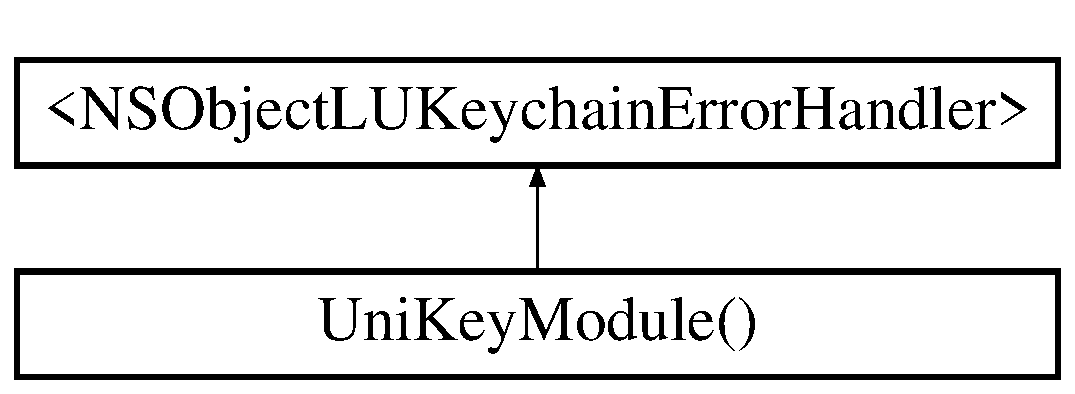
\includegraphics[height=2.000000cm]{category_uni_key_module_07_08}
\end{center}
\end{figure}
\subsection*{Properties}
\begin{DoxyCompactItemize}
\item 
\mbox{\Hypertarget{category_uni_key_module_07_08_a60acaad29a9f55a0833d1fb8ecd325cc}\label{category_uni_key_module_07_08_a60acaad29a9f55a0833d1fb8ecd325cc}} 
\mbox{\hyperlink{interface_l_u_keychain_access}{L\+U\+Keychain\+Access}} $\ast$ {\bfseries keychain\+Accesses}
\item 
N\+S\+Error $\ast$ \mbox{\hyperlink{category_uni_key_module_07_08_aa944f0b4ca37d1922b1c13d97903f3e8}{error}}
\end{DoxyCompactItemize}


\subsection{Property Documentation}
\mbox{\Hypertarget{category_uni_key_module_07_08_aa944f0b4ca37d1922b1c13d97903f3e8}\label{category_uni_key_module_07_08_aa944f0b4ca37d1922b1c13d97903f3e8}} 
\index{Uni\+Key\+Module()@{Uni\+Key\+Module()}!error@{error}}
\index{error@{error}!Uni\+Key\+Module()@{Uni\+Key\+Module()}}
\subsubsection{\texorpdfstring{error}{error}}
{\footnotesize\ttfamily -\/ (N\+S\+Error$\ast$) error\hspace{0.3cm}{\ttfamily [read]}, {\ttfamily [write]}, {\ttfamily [nonatomic]}, {\ttfamily [strong]}}

Error\+Code

If it occurred error while using keychain api, detailed errors reason will be recorded to this memory area. 

The documentation for this category was generated from the following file\+:\begin{DoxyCompactItemize}
\item 
Assets/\+Plugins/unikeymodule/i\+O\+S/Uni\+Key\+Module.\+mm\end{DoxyCompactItemize}

\hypertarget{struct_uni_key_module_boolean}{}\section{Uni\+Key\+Module\+Boolean Struct Reference}
\label{struct_uni_key_module_boolean}\index{Uni\+Key\+Module\+Boolean@{Uni\+Key\+Module\+Boolean}}
\subsection*{Public Attributes}
\begin{DoxyCompactItemize}
\item 
\mbox{\Hypertarget{struct_uni_key_module_boolean_a7afee4ddf3bebf409c905d637261137c}\label{struct_uni_key_module_boolean_a7afee4ddf3bebf409c905d637261137c}} 
bool {\bfseries value}
\item 
\mbox{\Hypertarget{struct_uni_key_module_boolean_acd72a7cfe27cfa86b28471e78cec74d9}\label{struct_uni_key_module_boolean_acd72a7cfe27cfa86b28471e78cec74d9}} 
int {\bfseries error\+Code}
\end{DoxyCompactItemize}


The documentation for this struct was generated from the following file\+:\begin{DoxyCompactItemize}
\item 
Assets/\+Plugins/unikeymodule/i\+O\+S/Uni\+Key\+Module.\+mm\end{DoxyCompactItemize}

\hypertarget{struct_siege_module_1_1_uni_key_module_boolean}{}\section{Siege\+Module.\+Uni\+Key\+Module\+Boolean Struct Reference}
\label{struct_siege_module_1_1_uni_key_module_boolean}\index{Siege\+Module.\+Uni\+Key\+Module\+Boolean@{Siege\+Module.\+Uni\+Key\+Module\+Boolean}}
\subsection*{Public Attributes}
\begin{DoxyCompactItemize}
\item 
bool \mbox{\hyperlink{struct_siege_module_1_1_uni_key_module_boolean_aeaf91918c514973225ad65bec8df4ac5}{value}}
\begin{DoxyCompactList}\small\item\em received boolean \end{DoxyCompactList}\item 
int \mbox{\hyperlink{struct_siege_module_1_1_uni_key_module_boolean_abbf053c46dcb1393a328bdd6049ab64c}{error\+Code}}
\begin{DoxyCompactList}\small\item\em received error code \end{DoxyCompactList}\end{DoxyCompactItemize}


\subsection{Member Data Documentation}
\mbox{\Hypertarget{struct_siege_module_1_1_uni_key_module_boolean_abbf053c46dcb1393a328bdd6049ab64c}\label{struct_siege_module_1_1_uni_key_module_boolean_abbf053c46dcb1393a328bdd6049ab64c}} 
\index{Siege\+Module\+::\+Uni\+Key\+Module\+Boolean@{Siege\+Module\+::\+Uni\+Key\+Module\+Boolean}!error\+Code@{error\+Code}}
\index{error\+Code@{error\+Code}!Siege\+Module\+::\+Uni\+Key\+Module\+Boolean@{Siege\+Module\+::\+Uni\+Key\+Module\+Boolean}}
\subsubsection{\texorpdfstring{error\+Code}{errorCode}}
{\footnotesize\ttfamily int Siege\+Module.\+Uni\+Key\+Module\+Boolean.\+error\+Code}



received error code 

\mbox{\Hypertarget{struct_siege_module_1_1_uni_key_module_boolean_aeaf91918c514973225ad65bec8df4ac5}\label{struct_siege_module_1_1_uni_key_module_boolean_aeaf91918c514973225ad65bec8df4ac5}} 
\index{Siege\+Module\+::\+Uni\+Key\+Module\+Boolean@{Siege\+Module\+::\+Uni\+Key\+Module\+Boolean}!value@{value}}
\index{value@{value}!Siege\+Module\+::\+Uni\+Key\+Module\+Boolean@{Siege\+Module\+::\+Uni\+Key\+Module\+Boolean}}
\subsubsection{\texorpdfstring{value}{value}}
{\footnotesize\ttfamily bool Siege\+Module.\+Uni\+Key\+Module\+Boolean.\+value}



received boolean 



The documentation for this struct was generated from the following file\+:\begin{DoxyCompactItemize}
\item 
Assets/\+Plugins/unikeymodule/Uni\+Key\+Module.\+cs\end{DoxyCompactItemize}

\hypertarget{class_siege_module_1_1_uni_key_module_build_processor}{}\section{Siege\+Module.\+Uni\+Key\+Module\+Build\+Processor Class Reference}
\label{class_siege_module_1_1_uni_key_module_build_processor}\index{Siege\+Module.\+Uni\+Key\+Module\+Build\+Processor@{Siege\+Module.\+Uni\+Key\+Module\+Build\+Processor}}
Inheritance diagram for Siege\+Module.\+Uni\+Key\+Module\+Build\+Processor\+:\begin{figure}[H]
\begin{center}
\leavevmode
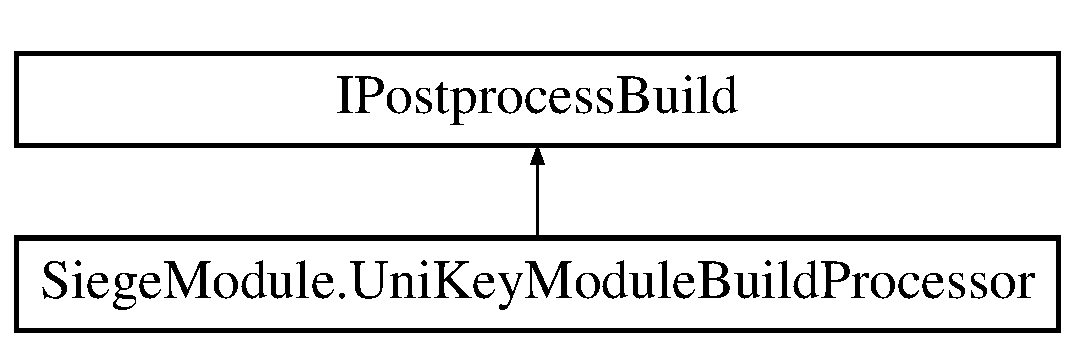
\includegraphics[height=2.000000cm]{class_siege_module_1_1_uni_key_module_build_processor}
\end{center}
\end{figure}
\subsection*{Properties}
\begin{DoxyCompactItemize}
\item 
int I\+Ordered\+Callback. \mbox{\hyperlink{class_siege_module_1_1_uni_key_module_build_processor_ac8a224393b5e14a918f7b83c11e52d4d}{callback\+Order}}\hspace{0.3cm}{\ttfamily  \mbox{[}get\mbox{]}}
\begin{DoxyCompactList}\small\item\em Order \end{DoxyCompactList}\end{DoxyCompactItemize}
\subsection*{Private Member Functions}
\begin{DoxyCompactItemize}
\item 
void I\+Postprocess\+Build. \mbox{\hyperlink{class_siege_module_1_1_uni_key_module_build_processor_a77a134492161b03b27b431bcfbf83011}{On\+Postprocess\+Build}} (Build\+Target target, string path)
\begin{DoxyCompactList}\small\item\em Post\+Process \end{DoxyCompactList}\end{DoxyCompactItemize}


\subsection{Member Function Documentation}
\mbox{\Hypertarget{class_siege_module_1_1_uni_key_module_build_processor_a77a134492161b03b27b431bcfbf83011}\label{class_siege_module_1_1_uni_key_module_build_processor_a77a134492161b03b27b431bcfbf83011}} 
\index{Siege\+Module\+::\+Uni\+Key\+Module\+Build\+Processor@{Siege\+Module\+::\+Uni\+Key\+Module\+Build\+Processor}!On\+Postprocess\+Build@{On\+Postprocess\+Build}}
\index{On\+Postprocess\+Build@{On\+Postprocess\+Build}!Siege\+Module\+::\+Uni\+Key\+Module\+Build\+Processor@{Siege\+Module\+::\+Uni\+Key\+Module\+Build\+Processor}}
\subsubsection{\texorpdfstring{On\+Postprocess\+Build()}{OnPostprocessBuild()}}
{\footnotesize\ttfamily void I\+Postprocess\+Build. Siege\+Module.\+Uni\+Key\+Module\+Build\+Processor.\+On\+Postprocess\+Build (\begin{DoxyParamCaption}\item[{Build\+Target}]{target,  }\item[{string}]{path }\end{DoxyParamCaption})\hspace{0.3cm}{\ttfamily [private]}}



Post\+Process 


\begin{DoxyParams}{Parameters}
{\em target} & \\
\hline
{\em path} & \\
\hline
\end{DoxyParams}


\subsection{Property Documentation}
\mbox{\Hypertarget{class_siege_module_1_1_uni_key_module_build_processor_ac8a224393b5e14a918f7b83c11e52d4d}\label{class_siege_module_1_1_uni_key_module_build_processor_ac8a224393b5e14a918f7b83c11e52d4d}} 
\index{Siege\+Module\+::\+Uni\+Key\+Module\+Build\+Processor@{Siege\+Module\+::\+Uni\+Key\+Module\+Build\+Processor}!callback\+Order@{callback\+Order}}
\index{callback\+Order@{callback\+Order}!Siege\+Module\+::\+Uni\+Key\+Module\+Build\+Processor@{Siege\+Module\+::\+Uni\+Key\+Module\+Build\+Processor}}
\subsubsection{\texorpdfstring{callback\+Order}{callbackOrder}}
{\footnotesize\ttfamily int I\+Ordered\+Callback. Siege\+Module.\+Uni\+Key\+Module\+Build\+Processor.\+callback\+Order\hspace{0.3cm}{\ttfamily [get]}, {\ttfamily [private]}}



Order 



The documentation for this class was generated from the following file\+:\begin{DoxyCompactItemize}
\item 
Assets/\+Plugins/unikeymodule/\+Editor/Uni\+Key\+Module\+Build\+Processor.\+cs\end{DoxyCompactItemize}

\hypertarget{class_siege_module_1_1_uni_key_module_exception}{}\section{Siege\+Module.\+Uni\+Key\+Module\+Exception Class Reference}
\label{class_siege_module_1_1_uni_key_module_exception}\index{Siege\+Module.\+Uni\+Key\+Module\+Exception@{Siege\+Module.\+Uni\+Key\+Module\+Exception}}


\mbox{\hyperlink{class_siege_module_1_1_uni_key_module}{Uni\+Key\+Module}} Original Exception  


Inheritance diagram for Siege\+Module.\+Uni\+Key\+Module\+Exception\+:\begin{figure}[H]
\begin{center}
\leavevmode
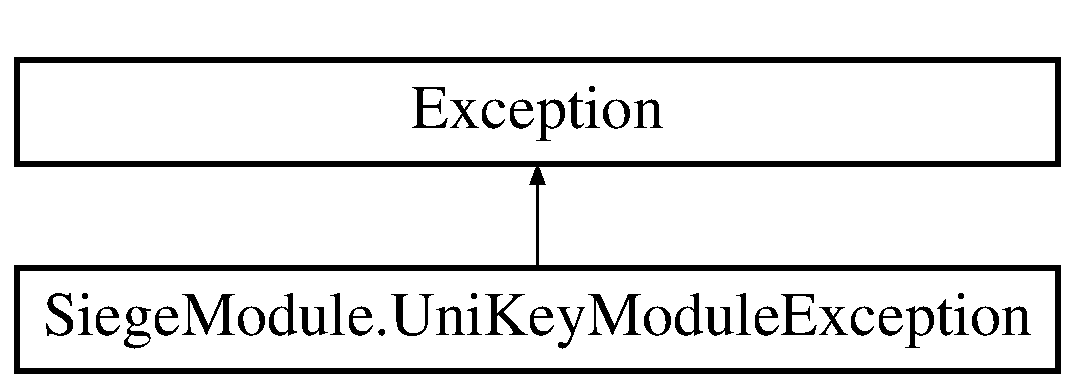
\includegraphics[height=2.000000cm]{class_siege_module_1_1_uni_key_module_exception}
\end{center}
\end{figure}
\subsection*{Public Member Functions}
\begin{DoxyCompactItemize}
\item 
\mbox{\hyperlink{class_siege_module_1_1_uni_key_module_exception_a0290bb9e9b14d83bdbe553c6a8a521f2}{Uni\+Key\+Module\+Exception}} (\mbox{\hyperlink{class_siege_module_1_1_uni_key_module_exception_ab0d37362fd3adf3ef985e3c5b8383be6}{Error\+Code}} error\+Code=Error\+Code.\+None)
\begin{DoxyCompactList}\small\item\em constructor \end{DoxyCompactList}\item 
\mbox{\hyperlink{class_siege_module_1_1_uni_key_module_exception_ab4d369837a09f843ff7b083844c9333c}{Uni\+Key\+Module\+Exception}} (string msg, \mbox{\hyperlink{class_siege_module_1_1_uni_key_module_exception_ab0d37362fd3adf3ef985e3c5b8383be6}{Error\+Code}} error\+Code=Error\+Code.\+None)
\begin{DoxyCompactList}\small\item\em constructor \end{DoxyCompactList}\item 
\mbox{\hyperlink{class_siege_module_1_1_uni_key_module_exception_af25eb96982f1282df0b7267e64be5915}{Uni\+Key\+Module\+Exception}} (string msg, Exception inner, \mbox{\hyperlink{class_siege_module_1_1_uni_key_module_exception_ab0d37362fd3adf3ef985e3c5b8383be6}{Error\+Code}} error\+Code=Error\+Code.\+None)
\begin{DoxyCompactList}\small\item\em constructor \end{DoxyCompactList}\end{DoxyCompactItemize}
\subsection*{Properties}
\begin{DoxyCompactItemize}
\item 
Error\+Code \mbox{\hyperlink{class_siege_module_1_1_uni_key_module_exception_ab0d37362fd3adf3ef985e3c5b8383be6}{Error\+Code}}\hspace{0.3cm}{\ttfamily  \mbox{[}get, private set\mbox{]}}
\begin{DoxyCompactList}\small\item\em error code \end{DoxyCompactList}\end{DoxyCompactItemize}


\subsection{Detailed Description}
\mbox{\hyperlink{class_siege_module_1_1_uni_key_module}{Uni\+Key\+Module}} Original Exception 



\subsection{Constructor \& Destructor Documentation}
\mbox{\Hypertarget{class_siege_module_1_1_uni_key_module_exception_a0290bb9e9b14d83bdbe553c6a8a521f2}\label{class_siege_module_1_1_uni_key_module_exception_a0290bb9e9b14d83bdbe553c6a8a521f2}} 
\index{Siege\+Module\+::\+Uni\+Key\+Module\+Exception@{Siege\+Module\+::\+Uni\+Key\+Module\+Exception}!Uni\+Key\+Module\+Exception@{Uni\+Key\+Module\+Exception}}
\index{Uni\+Key\+Module\+Exception@{Uni\+Key\+Module\+Exception}!Siege\+Module\+::\+Uni\+Key\+Module\+Exception@{Siege\+Module\+::\+Uni\+Key\+Module\+Exception}}
\subsubsection{\texorpdfstring{Uni\+Key\+Module\+Exception()}{UniKeyModuleException()}\hspace{0.1cm}{\footnotesize\ttfamily [1/3]}}
{\footnotesize\ttfamily Siege\+Module.\+Uni\+Key\+Module\+Exception.\+Uni\+Key\+Module\+Exception (\begin{DoxyParamCaption}\item[{\mbox{\hyperlink{class_siege_module_1_1_uni_key_module_exception_ab0d37362fd3adf3ef985e3c5b8383be6}{Error\+Code}}}]{error\+Code = {\ttfamily ErrorCode.None} }\end{DoxyParamCaption})}



constructor 


\begin{DoxyParams}{Parameters}
{\em error\+Code} & error\+Code\\
\hline
\end{DoxyParams}
\mbox{\Hypertarget{class_siege_module_1_1_uni_key_module_exception_ab4d369837a09f843ff7b083844c9333c}\label{class_siege_module_1_1_uni_key_module_exception_ab4d369837a09f843ff7b083844c9333c}} 
\index{Siege\+Module\+::\+Uni\+Key\+Module\+Exception@{Siege\+Module\+::\+Uni\+Key\+Module\+Exception}!Uni\+Key\+Module\+Exception@{Uni\+Key\+Module\+Exception}}
\index{Uni\+Key\+Module\+Exception@{Uni\+Key\+Module\+Exception}!Siege\+Module\+::\+Uni\+Key\+Module\+Exception@{Siege\+Module\+::\+Uni\+Key\+Module\+Exception}}
\subsubsection{\texorpdfstring{Uni\+Key\+Module\+Exception()}{UniKeyModuleException()}\hspace{0.1cm}{\footnotesize\ttfamily [2/3]}}
{\footnotesize\ttfamily Siege\+Module.\+Uni\+Key\+Module\+Exception.\+Uni\+Key\+Module\+Exception (\begin{DoxyParamCaption}\item[{string}]{msg,  }\item[{\mbox{\hyperlink{class_siege_module_1_1_uni_key_module_exception_ab0d37362fd3adf3ef985e3c5b8383be6}{Error\+Code}}}]{error\+Code = {\ttfamily ErrorCode.None} }\end{DoxyParamCaption})}



constructor 


\begin{DoxyParams}{Parameters}
{\em msg} & error\+Message\\
\hline
{\em error\+Code} & error\+Code\\
\hline
\end{DoxyParams}
\mbox{\Hypertarget{class_siege_module_1_1_uni_key_module_exception_af25eb96982f1282df0b7267e64be5915}\label{class_siege_module_1_1_uni_key_module_exception_af25eb96982f1282df0b7267e64be5915}} 
\index{Siege\+Module\+::\+Uni\+Key\+Module\+Exception@{Siege\+Module\+::\+Uni\+Key\+Module\+Exception}!Uni\+Key\+Module\+Exception@{Uni\+Key\+Module\+Exception}}
\index{Uni\+Key\+Module\+Exception@{Uni\+Key\+Module\+Exception}!Siege\+Module\+::\+Uni\+Key\+Module\+Exception@{Siege\+Module\+::\+Uni\+Key\+Module\+Exception}}
\subsubsection{\texorpdfstring{Uni\+Key\+Module\+Exception()}{UniKeyModuleException()}\hspace{0.1cm}{\footnotesize\ttfamily [3/3]}}
{\footnotesize\ttfamily Siege\+Module.\+Uni\+Key\+Module\+Exception.\+Uni\+Key\+Module\+Exception (\begin{DoxyParamCaption}\item[{string}]{msg,  }\item[{Exception}]{inner,  }\item[{\mbox{\hyperlink{class_siege_module_1_1_uni_key_module_exception_ab0d37362fd3adf3ef985e3c5b8383be6}{Error\+Code}}}]{error\+Code = {\ttfamily ErrorCode.None} }\end{DoxyParamCaption})}



constructor 


\begin{DoxyParams}{Parameters}
{\em msg} & error\+Message\\
\hline
{\em inner} & exception\\
\hline
{\em error\+Code} & error\+Code\\
\hline
\end{DoxyParams}


\subsection{Property Documentation}
\mbox{\Hypertarget{class_siege_module_1_1_uni_key_module_exception_ab0d37362fd3adf3ef985e3c5b8383be6}\label{class_siege_module_1_1_uni_key_module_exception_ab0d37362fd3adf3ef985e3c5b8383be6}} 
\index{Siege\+Module\+::\+Uni\+Key\+Module\+Exception@{Siege\+Module\+::\+Uni\+Key\+Module\+Exception}!Error\+Code@{Error\+Code}}
\index{Error\+Code@{Error\+Code}!Siege\+Module\+::\+Uni\+Key\+Module\+Exception@{Siege\+Module\+::\+Uni\+Key\+Module\+Exception}}
\subsubsection{\texorpdfstring{Error\+Code}{ErrorCode}}
{\footnotesize\ttfamily Error\+Code Siege\+Module.\+Uni\+Key\+Module\+Exception.\+Error\+Code\hspace{0.3cm}{\ttfamily [get]}, {\ttfamily [private set]}}



error code 



The documentation for this class was generated from the following file\+:\begin{DoxyCompactItemize}
\item 
Assets/\+Plugins/unikeymodule/Uni\+Key\+Module\+Exception.\+cs\end{DoxyCompactItemize}

\hypertarget{class_siege_module_1_1_uni_key_module_other}{}\section{Siege\+Module.\+Uni\+Key\+Module\+Other Class Reference}
\label{class_siege_module_1_1_uni_key_module_other}\index{Siege\+Module.\+Uni\+Key\+Module\+Other@{Siege\+Module.\+Uni\+Key\+Module\+Other}}
\subsection*{Classes}
\begin{DoxyCompactItemize}
\item 
struct \mbox{\hyperlink{struct_siege_module_1_1_uni_key_module_other_1_1_k_v}{KV}}
\begin{DoxyCompactList}\small\item\em key-\/value data structure. \end{DoxyCompactList}\end{DoxyCompactItemize}
\subsection*{Static Public Member Functions}
\begin{DoxyCompactItemize}
\item 
static \mbox{\hyperlink{struct_siege_module_1_1_uni_key_module_string}{Uni\+Key\+Module\+String}} \mbox{\hyperlink{class_siege_module_1_1_uni_key_module_other_af31fe254c5de6ef3f85001865801d0af}{Get\+String}} (string key)
\begin{DoxyCompactList}\small\item\em get value from cache. \end{DoxyCompactList}\item 
static int \mbox{\hyperlink{class_siege_module_1_1_uni_key_module_other_a3c863fcdc7762d02692f88f18240ed4c}{Set\+String}} (string key, string value)
\begin{DoxyCompactList}\small\item\em set value to cache and xml. \end{DoxyCompactList}\item 
static \mbox{\hyperlink{struct_siege_module_1_1_uni_key_module_boolean}{Uni\+Key\+Module\+Boolean}} \mbox{\hyperlink{class_siege_module_1_1_uni_key_module_other_adb8428817e6364d8cf1417c8806f9b80}{Has\+Key}} (string key)
\begin{DoxyCompactList}\small\item\em confirm that cache contains key \end{DoxyCompactList}\item 
static Error\+Code \mbox{\hyperlink{class_siege_module_1_1_uni_key_module_other_a273d7ae437e207ed153e5233e0887297}{Delete\+Key}} (string key)
\begin{DoxyCompactList}\small\item\em delete a data from cache and xml. \end{DoxyCompactList}\item 
static int \mbox{\hyperlink{class_siege_module_1_1_uni_key_module_other_adc5fcb32fc28119ca512c842f11d1d12}{Delete\+All}} ()
\begin{DoxyCompactList}\small\item\em delete all data from cache and xml. \end{DoxyCompactList}\end{DoxyCompactItemize}
\subsection*{Static Private Member Functions}
\begin{DoxyCompactItemize}
\item 
static \mbox{\hyperlink{class_siege_module_1_1_uni_key_module_other_ab7a64f84ab192cb186c60116b65d4c4b}{Uni\+Key\+Module\+Other}} ()
\begin{DoxyCompactList}\small\item\em static constructor when program is starting, it deserialize data from xml-\/file, if xml-\/file existed. \end{DoxyCompactList}\item 
static void \mbox{\hyperlink{class_siege_module_1_1_uni_key_module_other_a9edb18f38f81b27348138c8cd13ead32}{Serialize}} ()
\begin{DoxyCompactList}\small\item\em serialize cache and create xml file. \end{DoxyCompactList}\item 
static void \mbox{\hyperlink{class_siege_module_1_1_uni_key_module_other_a705e91fd483e35dee3dca4328ec1c939}{Deserialize}} ()
\begin{DoxyCompactList}\small\item\em deserialize xml file and arrange to cache. \end{DoxyCompactList}\item 
static string \mbox{\hyperlink{class_siege_module_1_1_uni_key_module_other_a5fd17dc4ef93fddb66a5d47d48fd5e0c}{Get\+File\+Path}} ()
\begin{DoxyCompactList}\small\item\em get path about destination xml file. \end{DoxyCompactList}\end{DoxyCompactItemize}
\subsection*{Static Private Attributes}
\begin{DoxyCompactItemize}
\item 
static List$<$ \mbox{\hyperlink{struct_siege_module_1_1_uni_key_module_other_1_1_k_v}{KV}} $>$ \mbox{\hyperlink{class_siege_module_1_1_uni_key_module_other_ad7b2adc7e9aae7e1bce9cda54ffd4f40}{cache}} = new List$<$\mbox{\hyperlink{struct_siege_module_1_1_uni_key_module_other_1_1_k_v}{KV}}$>$()
\begin{DoxyCompactList}\small\item\em cache on memory. \end{DoxyCompactList}\end{DoxyCompactItemize}


\subsection{Constructor \& Destructor Documentation}
\mbox{\Hypertarget{class_siege_module_1_1_uni_key_module_other_ab7a64f84ab192cb186c60116b65d4c4b}\label{class_siege_module_1_1_uni_key_module_other_ab7a64f84ab192cb186c60116b65d4c4b}} 
\index{Siege\+Module\+::\+Uni\+Key\+Module\+Other@{Siege\+Module\+::\+Uni\+Key\+Module\+Other}!Uni\+Key\+Module\+Other@{Uni\+Key\+Module\+Other}}
\index{Uni\+Key\+Module\+Other@{Uni\+Key\+Module\+Other}!Siege\+Module\+::\+Uni\+Key\+Module\+Other@{Siege\+Module\+::\+Uni\+Key\+Module\+Other}}
\subsubsection{\texorpdfstring{Uni\+Key\+Module\+Other()}{UniKeyModuleOther()}}
{\footnotesize\ttfamily static Siege\+Module.\+Uni\+Key\+Module\+Other.\+Uni\+Key\+Module\+Other (\begin{DoxyParamCaption}{ }\end{DoxyParamCaption})\hspace{0.3cm}{\ttfamily [static]}, {\ttfamily [private]}}



static constructor when program is starting, it deserialize data from xml-\/file, if xml-\/file existed. 



\subsection{Member Function Documentation}
\mbox{\Hypertarget{class_siege_module_1_1_uni_key_module_other_adc5fcb32fc28119ca512c842f11d1d12}\label{class_siege_module_1_1_uni_key_module_other_adc5fcb32fc28119ca512c842f11d1d12}} 
\index{Siege\+Module\+::\+Uni\+Key\+Module\+Other@{Siege\+Module\+::\+Uni\+Key\+Module\+Other}!Delete\+All@{Delete\+All}}
\index{Delete\+All@{Delete\+All}!Siege\+Module\+::\+Uni\+Key\+Module\+Other@{Siege\+Module\+::\+Uni\+Key\+Module\+Other}}
\subsubsection{\texorpdfstring{Delete\+All()}{DeleteAll()}}
{\footnotesize\ttfamily static int Siege\+Module.\+Uni\+Key\+Module\+Other.\+Delete\+All (\begin{DoxyParamCaption}{ }\end{DoxyParamCaption})\hspace{0.3cm}{\ttfamily [static]}}



delete all data from cache and xml. 

\begin{DoxyReturn}{Returns}
error code
\end{DoxyReturn}
\mbox{\Hypertarget{class_siege_module_1_1_uni_key_module_other_a273d7ae437e207ed153e5233e0887297}\label{class_siege_module_1_1_uni_key_module_other_a273d7ae437e207ed153e5233e0887297}} 
\index{Siege\+Module\+::\+Uni\+Key\+Module\+Other@{Siege\+Module\+::\+Uni\+Key\+Module\+Other}!Delete\+Key@{Delete\+Key}}
\index{Delete\+Key@{Delete\+Key}!Siege\+Module\+::\+Uni\+Key\+Module\+Other@{Siege\+Module\+::\+Uni\+Key\+Module\+Other}}
\subsubsection{\texorpdfstring{Delete\+Key()}{DeleteKey()}}
{\footnotesize\ttfamily static Error\+Code Siege\+Module.\+Uni\+Key\+Module\+Other.\+Delete\+Key (\begin{DoxyParamCaption}\item[{string}]{key }\end{DoxyParamCaption})\hspace{0.3cm}{\ttfamily [static]}}



delete a data from cache and xml. 

\begin{DoxyReturn}{Returns}
error code
\end{DoxyReturn}

\begin{DoxyParams}{Parameters}
{\em key} & key\\
\hline
\end{DoxyParams}
\mbox{\Hypertarget{class_siege_module_1_1_uni_key_module_other_a705e91fd483e35dee3dca4328ec1c939}\label{class_siege_module_1_1_uni_key_module_other_a705e91fd483e35dee3dca4328ec1c939}} 
\index{Siege\+Module\+::\+Uni\+Key\+Module\+Other@{Siege\+Module\+::\+Uni\+Key\+Module\+Other}!Deserialize@{Deserialize}}
\index{Deserialize@{Deserialize}!Siege\+Module\+::\+Uni\+Key\+Module\+Other@{Siege\+Module\+::\+Uni\+Key\+Module\+Other}}
\subsubsection{\texorpdfstring{Deserialize()}{Deserialize()}}
{\footnotesize\ttfamily static void Siege\+Module.\+Uni\+Key\+Module\+Other.\+Deserialize (\begin{DoxyParamCaption}{ }\end{DoxyParamCaption})\hspace{0.3cm}{\ttfamily [static]}, {\ttfamily [private]}}



deserialize xml file and arrange to cache. 

\mbox{\Hypertarget{class_siege_module_1_1_uni_key_module_other_a5fd17dc4ef93fddb66a5d47d48fd5e0c}\label{class_siege_module_1_1_uni_key_module_other_a5fd17dc4ef93fddb66a5d47d48fd5e0c}} 
\index{Siege\+Module\+::\+Uni\+Key\+Module\+Other@{Siege\+Module\+::\+Uni\+Key\+Module\+Other}!Get\+File\+Path@{Get\+File\+Path}}
\index{Get\+File\+Path@{Get\+File\+Path}!Siege\+Module\+::\+Uni\+Key\+Module\+Other@{Siege\+Module\+::\+Uni\+Key\+Module\+Other}}
\subsubsection{\texorpdfstring{Get\+File\+Path()}{GetFilePath()}}
{\footnotesize\ttfamily static string Siege\+Module.\+Uni\+Key\+Module\+Other.\+Get\+File\+Path (\begin{DoxyParamCaption}{ }\end{DoxyParamCaption})\hspace{0.3cm}{\ttfamily [static]}, {\ttfamily [private]}}



get path about destination xml file. 

\begin{DoxyReturn}{Returns}
file path
\end{DoxyReturn}
\mbox{\Hypertarget{class_siege_module_1_1_uni_key_module_other_af31fe254c5de6ef3f85001865801d0af}\label{class_siege_module_1_1_uni_key_module_other_af31fe254c5de6ef3f85001865801d0af}} 
\index{Siege\+Module\+::\+Uni\+Key\+Module\+Other@{Siege\+Module\+::\+Uni\+Key\+Module\+Other}!Get\+String@{Get\+String}}
\index{Get\+String@{Get\+String}!Siege\+Module\+::\+Uni\+Key\+Module\+Other@{Siege\+Module\+::\+Uni\+Key\+Module\+Other}}
\subsubsection{\texorpdfstring{Get\+String()}{GetString()}}
{\footnotesize\ttfamily static \mbox{\hyperlink{struct_siege_module_1_1_uni_key_module_string}{Uni\+Key\+Module\+String}} Siege\+Module.\+Uni\+Key\+Module\+Other.\+Get\+String (\begin{DoxyParamCaption}\item[{string}]{key }\end{DoxyParamCaption})\hspace{0.3cm}{\ttfamily [static]}}



get value from cache. 

\begin{DoxyReturn}{Returns}
value + error code.
\end{DoxyReturn}

\begin{DoxyParams}{Parameters}
{\em key} & key\\
\hline
\end{DoxyParams}
\mbox{\Hypertarget{class_siege_module_1_1_uni_key_module_other_adb8428817e6364d8cf1417c8806f9b80}\label{class_siege_module_1_1_uni_key_module_other_adb8428817e6364d8cf1417c8806f9b80}} 
\index{Siege\+Module\+::\+Uni\+Key\+Module\+Other@{Siege\+Module\+::\+Uni\+Key\+Module\+Other}!Has\+Key@{Has\+Key}}
\index{Has\+Key@{Has\+Key}!Siege\+Module\+::\+Uni\+Key\+Module\+Other@{Siege\+Module\+::\+Uni\+Key\+Module\+Other}}
\subsubsection{\texorpdfstring{Has\+Key()}{HasKey()}}
{\footnotesize\ttfamily static \mbox{\hyperlink{struct_siege_module_1_1_uni_key_module_boolean}{Uni\+Key\+Module\+Boolean}} Siege\+Module.\+Uni\+Key\+Module\+Other.\+Has\+Key (\begin{DoxyParamCaption}\item[{string}]{key }\end{DoxyParamCaption})\hspace{0.3cm}{\ttfamily [static]}}



confirm that cache contains key 

\begin{DoxyReturn}{Returns}
value + error code
\end{DoxyReturn}

\begin{DoxyParams}{Parameters}
{\em key} & key\\
\hline
\end{DoxyParams}
\mbox{\Hypertarget{class_siege_module_1_1_uni_key_module_other_a9edb18f38f81b27348138c8cd13ead32}\label{class_siege_module_1_1_uni_key_module_other_a9edb18f38f81b27348138c8cd13ead32}} 
\index{Siege\+Module\+::\+Uni\+Key\+Module\+Other@{Siege\+Module\+::\+Uni\+Key\+Module\+Other}!Serialize@{Serialize}}
\index{Serialize@{Serialize}!Siege\+Module\+::\+Uni\+Key\+Module\+Other@{Siege\+Module\+::\+Uni\+Key\+Module\+Other}}
\subsubsection{\texorpdfstring{Serialize()}{Serialize()}}
{\footnotesize\ttfamily static void Siege\+Module.\+Uni\+Key\+Module\+Other.\+Serialize (\begin{DoxyParamCaption}{ }\end{DoxyParamCaption})\hspace{0.3cm}{\ttfamily [static]}, {\ttfamily [private]}}



serialize cache and create xml file. 

\mbox{\Hypertarget{class_siege_module_1_1_uni_key_module_other_a3c863fcdc7762d02692f88f18240ed4c}\label{class_siege_module_1_1_uni_key_module_other_a3c863fcdc7762d02692f88f18240ed4c}} 
\index{Siege\+Module\+::\+Uni\+Key\+Module\+Other@{Siege\+Module\+::\+Uni\+Key\+Module\+Other}!Set\+String@{Set\+String}}
\index{Set\+String@{Set\+String}!Siege\+Module\+::\+Uni\+Key\+Module\+Other@{Siege\+Module\+::\+Uni\+Key\+Module\+Other}}
\subsubsection{\texorpdfstring{Set\+String()}{SetString()}}
{\footnotesize\ttfamily static int Siege\+Module.\+Uni\+Key\+Module\+Other.\+Set\+String (\begin{DoxyParamCaption}\item[{string}]{key,  }\item[{string}]{value }\end{DoxyParamCaption})\hspace{0.3cm}{\ttfamily [static]}}



set value to cache and xml. 

\begin{DoxyReturn}{Returns}
error code
\end{DoxyReturn}

\begin{DoxyParams}{Parameters}
{\em key} & key\\
\hline
{\em value} & value\\
\hline
\end{DoxyParams}


\subsection{Member Data Documentation}
\mbox{\Hypertarget{class_siege_module_1_1_uni_key_module_other_ad7b2adc7e9aae7e1bce9cda54ffd4f40}\label{class_siege_module_1_1_uni_key_module_other_ad7b2adc7e9aae7e1bce9cda54ffd4f40}} 
\index{Siege\+Module\+::\+Uni\+Key\+Module\+Other@{Siege\+Module\+::\+Uni\+Key\+Module\+Other}!cache@{cache}}
\index{cache@{cache}!Siege\+Module\+::\+Uni\+Key\+Module\+Other@{Siege\+Module\+::\+Uni\+Key\+Module\+Other}}
\subsubsection{\texorpdfstring{cache}{cache}}
{\footnotesize\ttfamily List$<$\mbox{\hyperlink{struct_siege_module_1_1_uni_key_module_other_1_1_k_v}{KV}}$>$ Siege\+Module.\+Uni\+Key\+Module\+Other.\+cache = new List$<$\mbox{\hyperlink{struct_siege_module_1_1_uni_key_module_other_1_1_k_v}{KV}}$>$()\hspace{0.3cm}{\ttfamily [static]}, {\ttfamily [private]}}



cache on memory. 



The documentation for this class was generated from the following file\+:\begin{DoxyCompactItemize}
\item 
Assets/\+Plugins/unikeymodule/\+Other/Uni\+Key\+Module\+Other.\+cs\end{DoxyCompactItemize}

\hypertarget{struct_siege_module_1_1_uni_key_module_string}{}\section{Siege\+Module.\+Uni\+Key\+Module\+String Struct Reference}
\label{struct_siege_module_1_1_uni_key_module_string}\index{Siege\+Module.\+Uni\+Key\+Module\+String@{Siege\+Module.\+Uni\+Key\+Module\+String}}
\subsection*{Public Attributes}
\begin{DoxyCompactItemize}
\item 
string \mbox{\hyperlink{struct_siege_module_1_1_uni_key_module_string_a0e7f26f2e39fa1f1cc0501a5936add2c}{value}}
\begin{DoxyCompactList}\small\item\em received string \end{DoxyCompactList}\item 
int \mbox{\hyperlink{struct_siege_module_1_1_uni_key_module_string_a7417d6c1dedd944789d0205ff2dabdf3}{error\+Code}}
\begin{DoxyCompactList}\small\item\em received error code \end{DoxyCompactList}\end{DoxyCompactItemize}


\subsection{Member Data Documentation}
\mbox{\Hypertarget{struct_siege_module_1_1_uni_key_module_string_a7417d6c1dedd944789d0205ff2dabdf3}\label{struct_siege_module_1_1_uni_key_module_string_a7417d6c1dedd944789d0205ff2dabdf3}} 
\index{Siege\+Module\+::\+Uni\+Key\+Module\+String@{Siege\+Module\+::\+Uni\+Key\+Module\+String}!error\+Code@{error\+Code}}
\index{error\+Code@{error\+Code}!Siege\+Module\+::\+Uni\+Key\+Module\+String@{Siege\+Module\+::\+Uni\+Key\+Module\+String}}
\subsubsection{\texorpdfstring{error\+Code}{errorCode}}
{\footnotesize\ttfamily int Siege\+Module.\+Uni\+Key\+Module\+String.\+error\+Code}



received error code 

\mbox{\Hypertarget{struct_siege_module_1_1_uni_key_module_string_a0e7f26f2e39fa1f1cc0501a5936add2c}\label{struct_siege_module_1_1_uni_key_module_string_a0e7f26f2e39fa1f1cc0501a5936add2c}} 
\index{Siege\+Module\+::\+Uni\+Key\+Module\+String@{Siege\+Module\+::\+Uni\+Key\+Module\+String}!value@{value}}
\index{value@{value}!Siege\+Module\+::\+Uni\+Key\+Module\+String@{Siege\+Module\+::\+Uni\+Key\+Module\+String}}
\subsubsection{\texorpdfstring{value}{value}}
{\footnotesize\ttfamily string Siege\+Module.\+Uni\+Key\+Module\+String.\+value}



received string 



The documentation for this struct was generated from the following file\+:\begin{DoxyCompactItemize}
\item 
Assets/\+Plugins/unikeymodule/Uni\+Key\+Module.\+cs\end{DoxyCompactItemize}

\hypertarget{struct_uni_key_module_string}{}\section{Uni\+Key\+Module\+String Struct Reference}
\label{struct_uni_key_module_string}\index{Uni\+Key\+Module\+String@{Uni\+Key\+Module\+String}}
\subsection*{Public Attributes}
\begin{DoxyCompactItemize}
\item 
\mbox{\Hypertarget{struct_uni_key_module_string_aec198910aabea29a9ca400778423cf5f}\label{struct_uni_key_module_string_aec198910aabea29a9ca400778423cf5f}} 
char $\ast$ {\bfseries value}
\item 
\mbox{\Hypertarget{struct_uni_key_module_string_a1e5a8b52fb256362d7f5b3655d964e4c}\label{struct_uni_key_module_string_a1e5a8b52fb256362d7f5b3655d964e4c}} 
int {\bfseries error\+Code}
\end{DoxyCompactItemize}


The documentation for this struct was generated from the following file\+:\begin{DoxyCompactItemize}
\item 
Assets/\+Plugins/unikeymodule/i\+O\+S/Uni\+Key\+Module.\+mm\end{DoxyCompactItemize}

%--- End generated contents ---

% Index
\backmatter
\newpage
\phantomsection
\clearemptydoublepage
\addcontentsline{toc}{chapter}{Index}
\printindex

\end{document}
